\chapter{Methodology}

\section{\textit{RangeCIR} dataset}\label{data_collection}

\begin{figure}[tbh]
    \centering
    \subfloat[Dataset collection environment]{%
        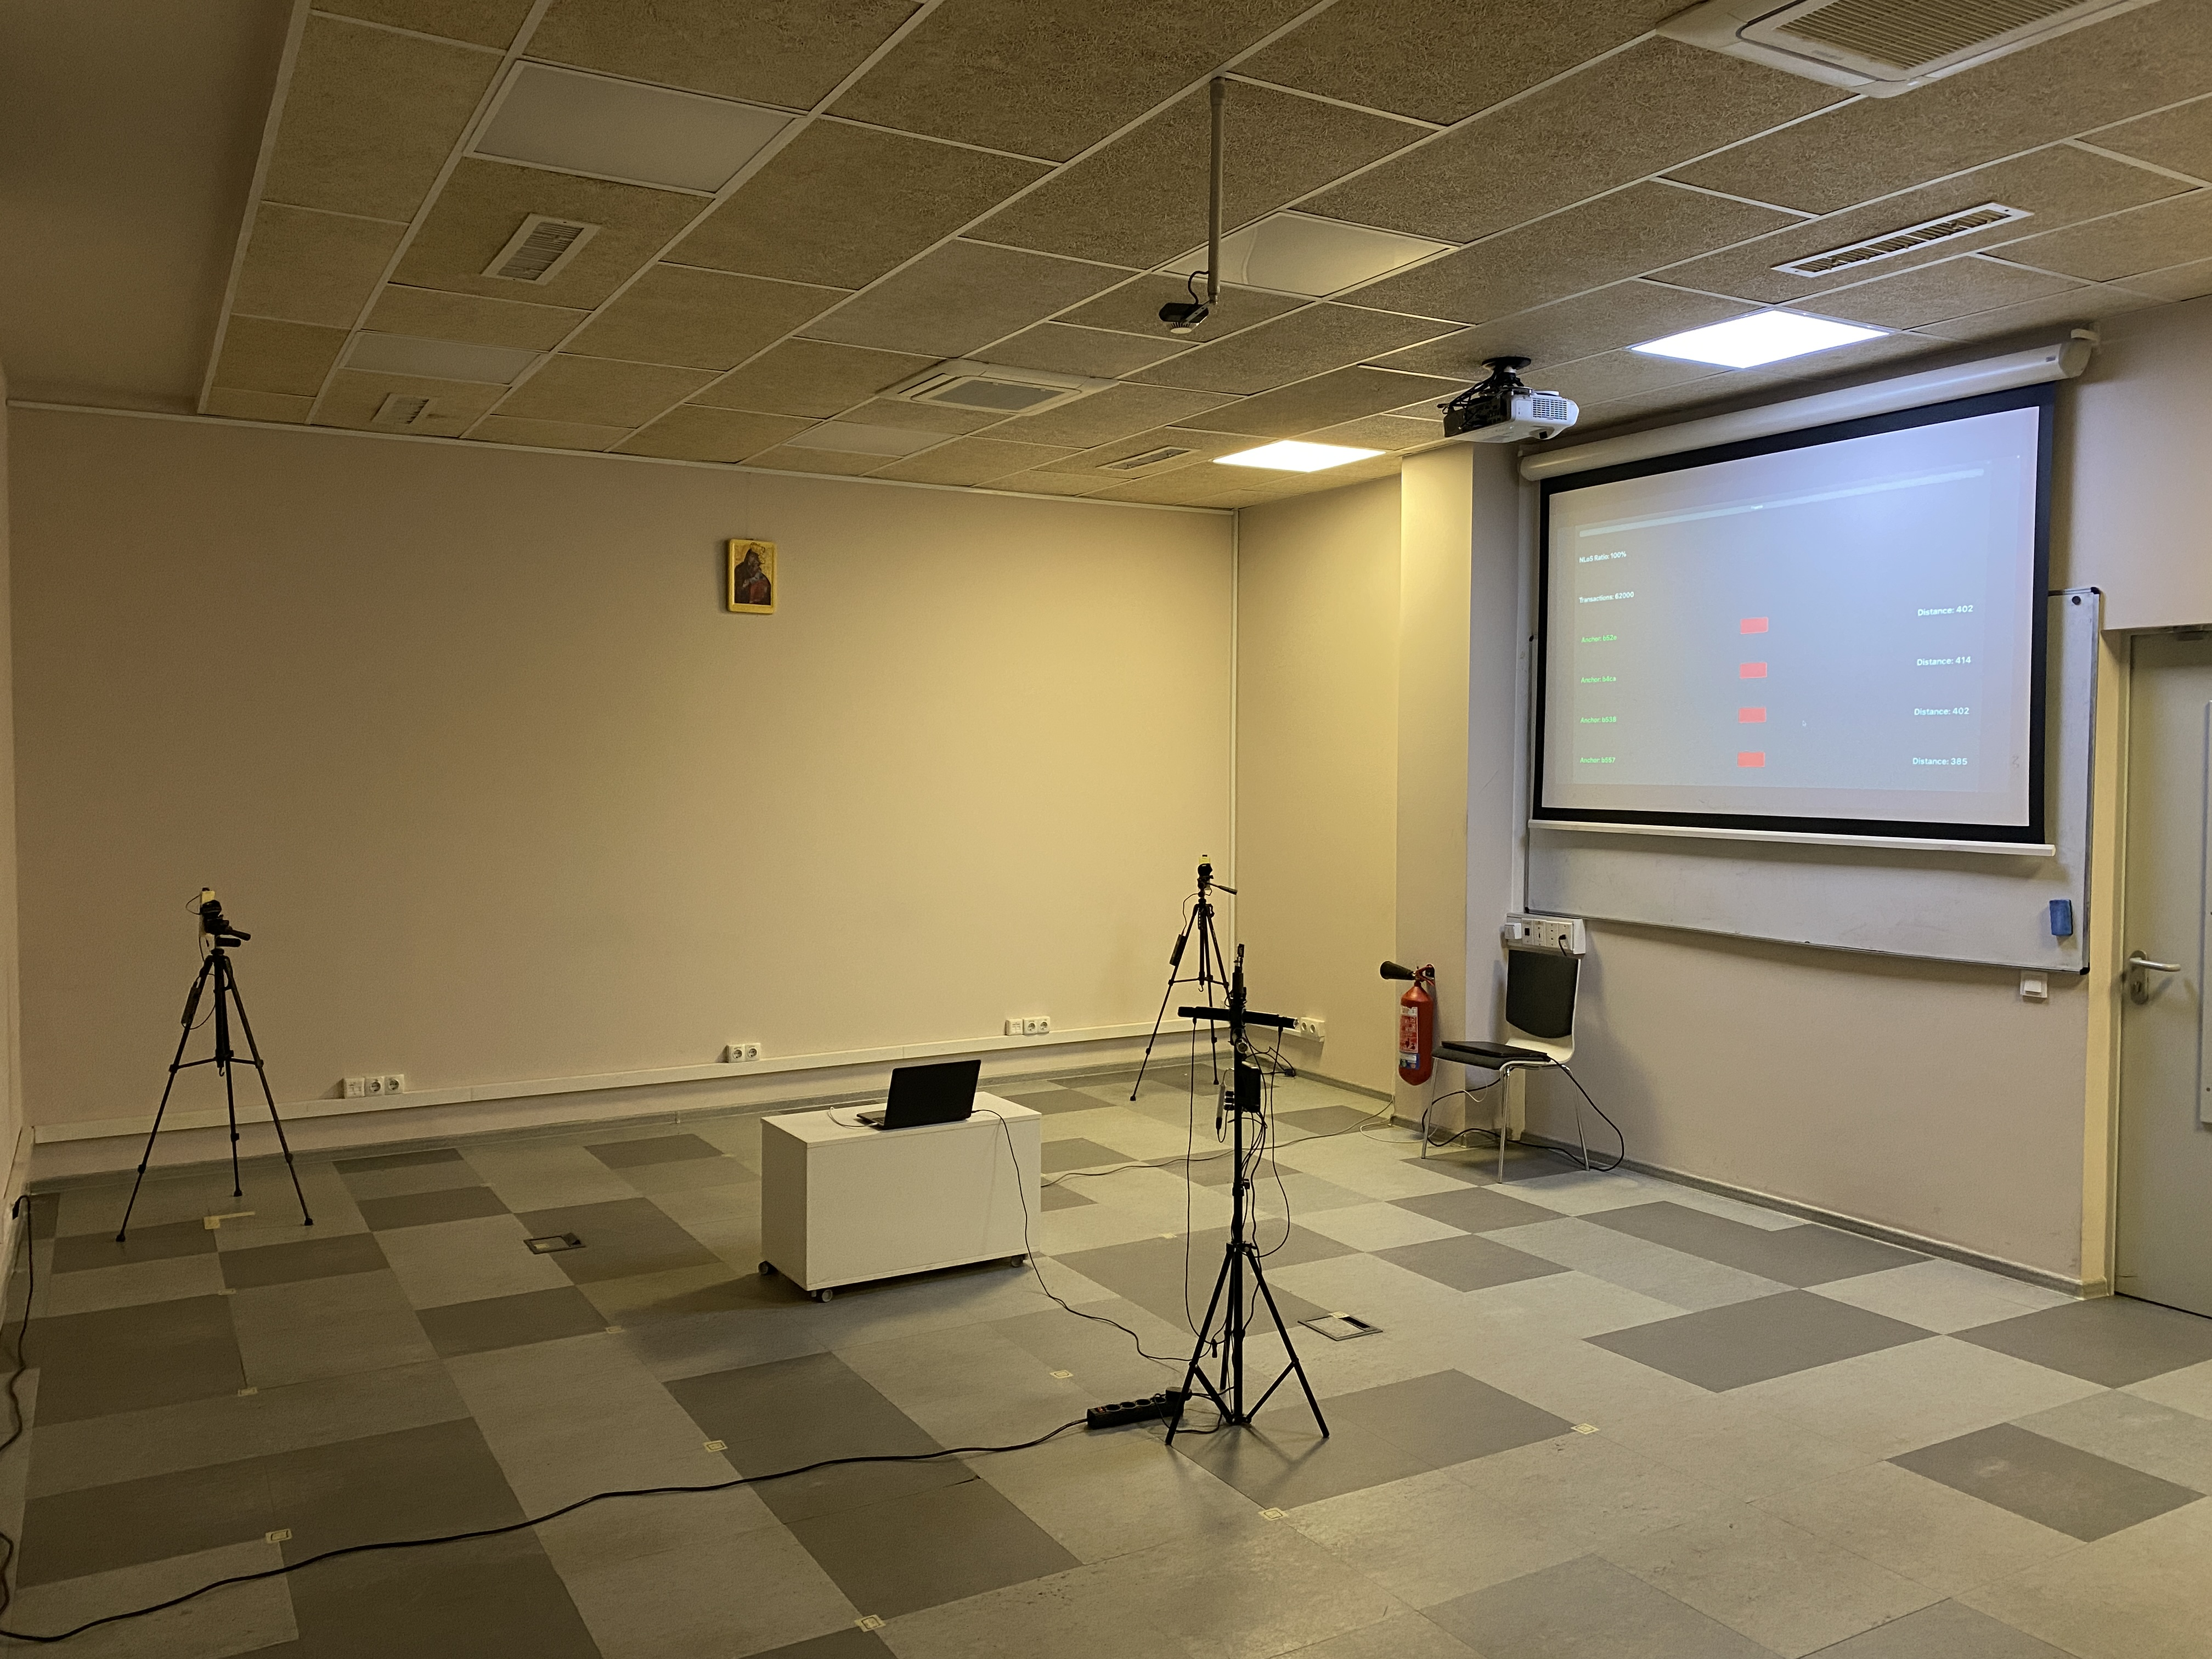
\includegraphics[height=6.5cm]{Figures/methodology/dataset_env.png}
        \label{fig:environment}
    }
    \subfloat[UWB Tag][UWB Tag]{%
        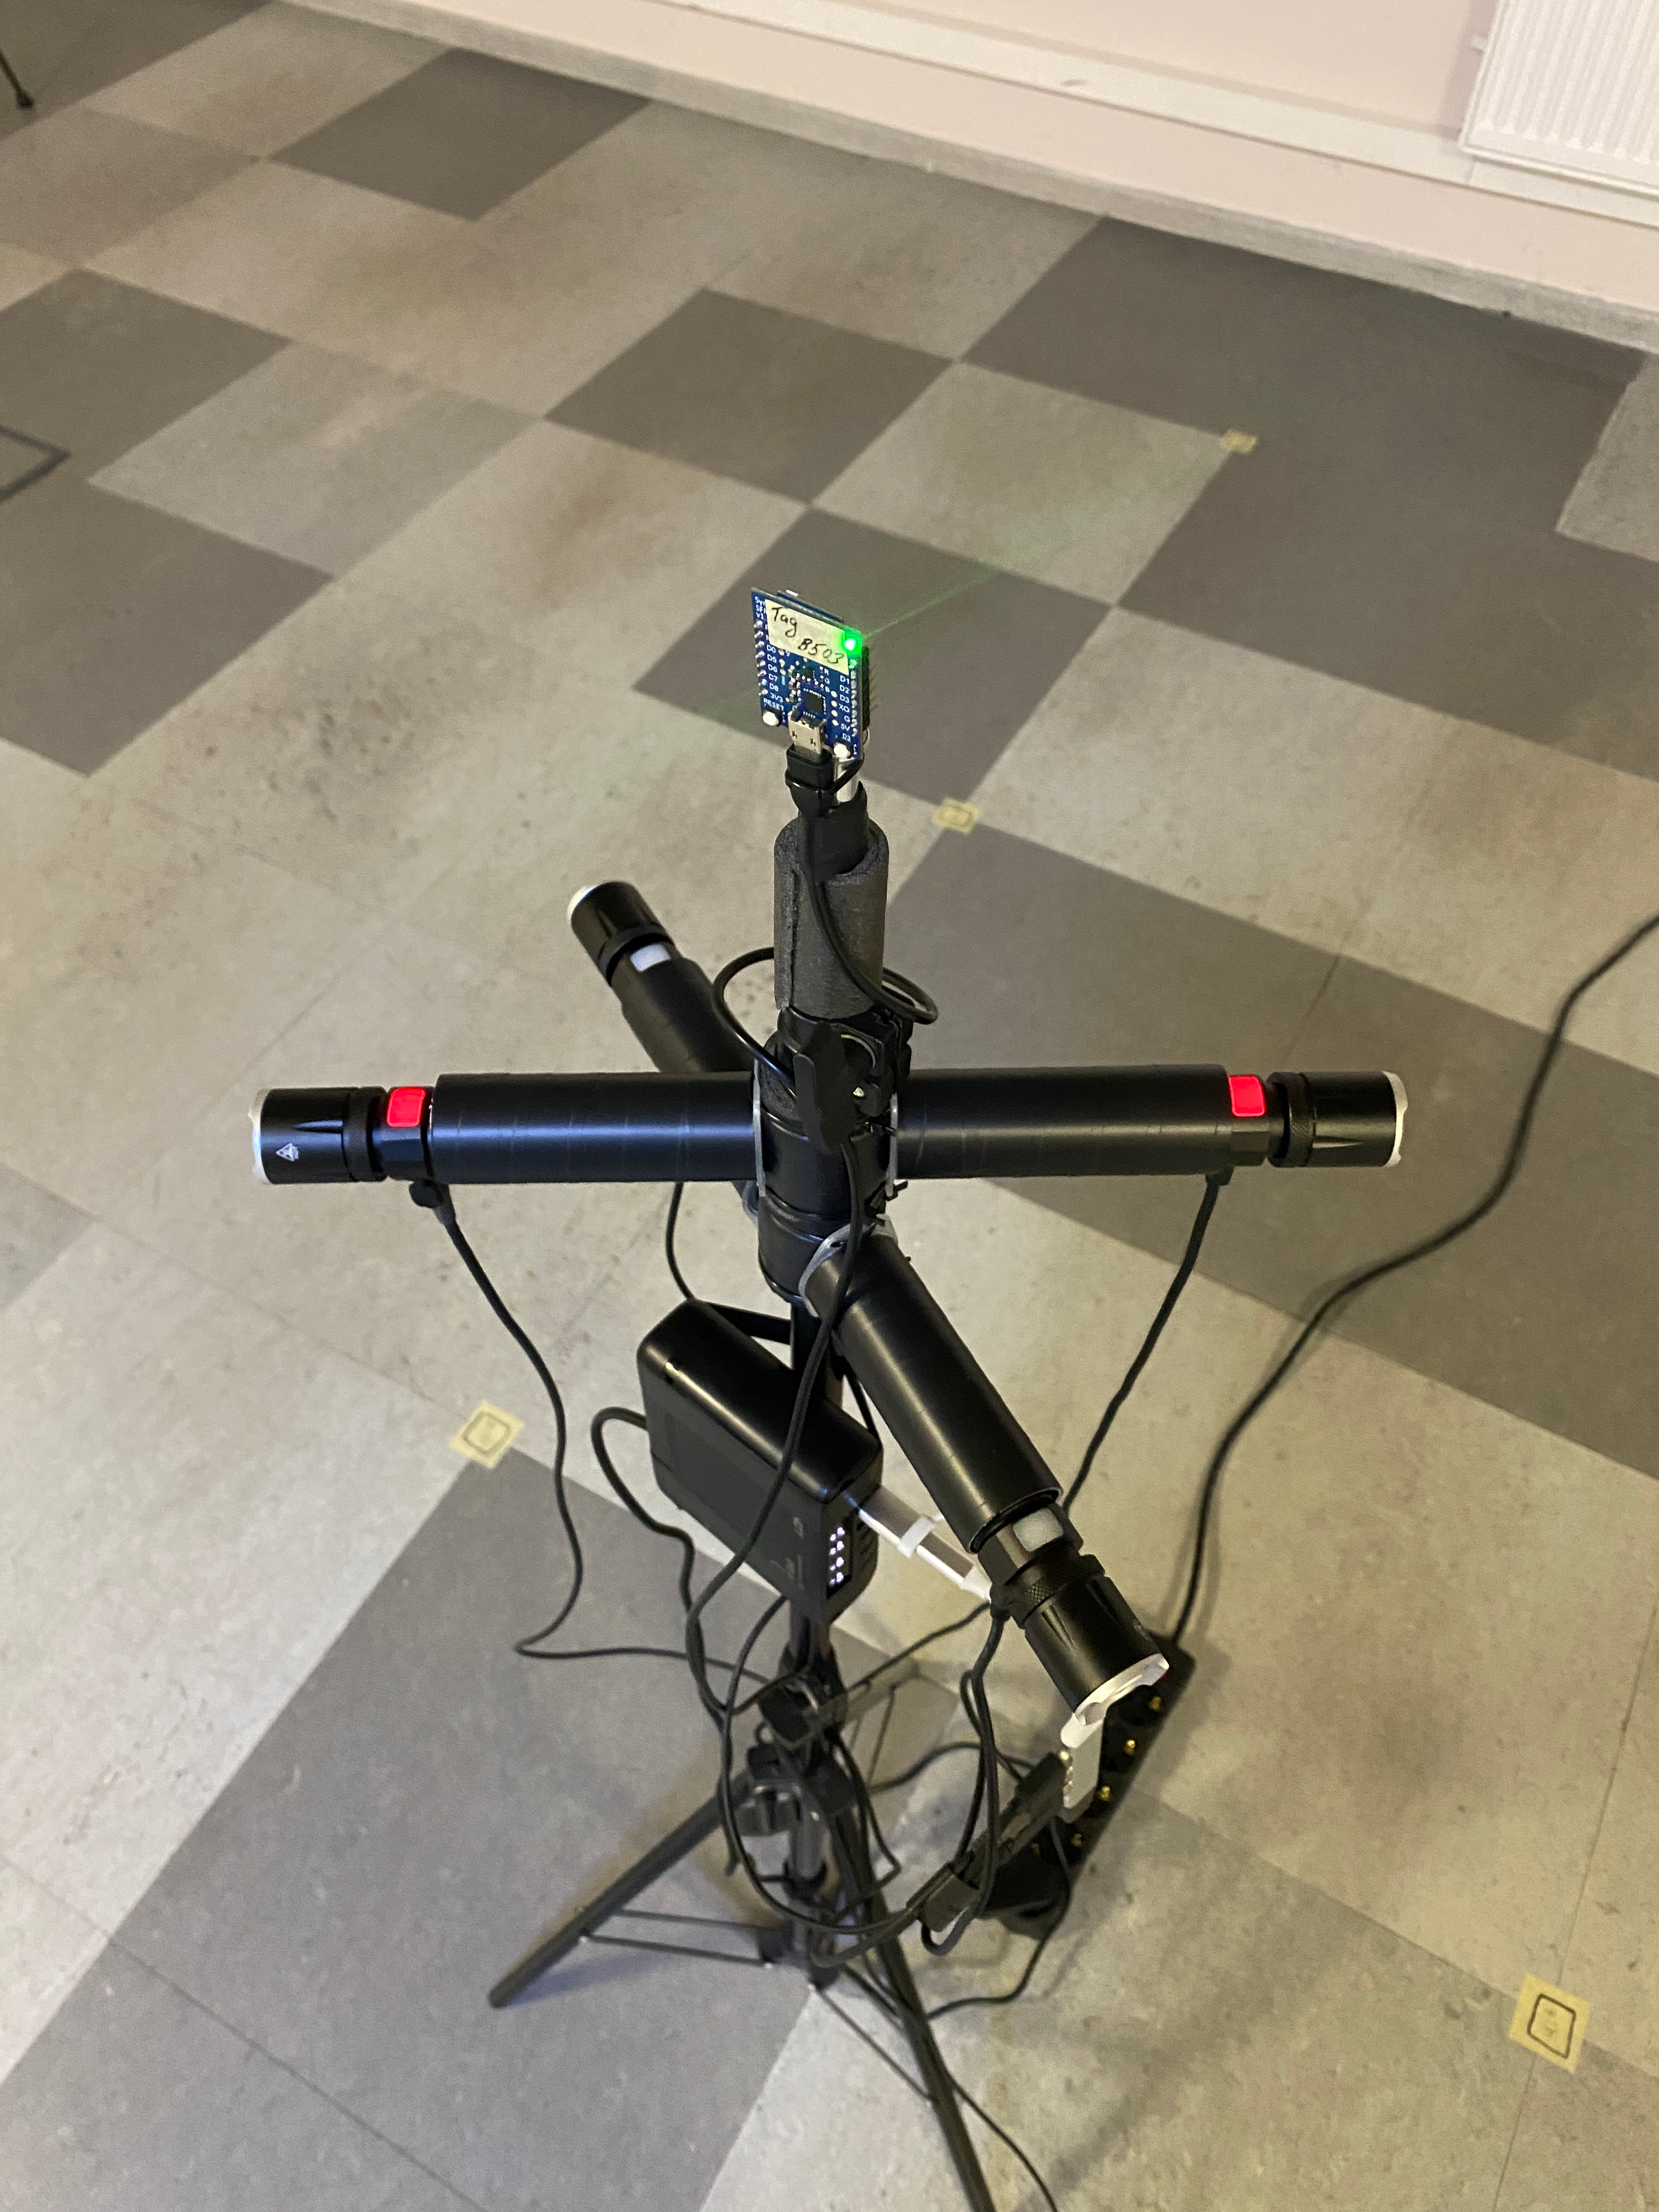
\includegraphics[height=6.5cm]{Figures/methodology/tag.png}
        \label{fig:tag}
    }
    \caption{Dataset collection environment.}
    \label{fig:dataset_setup}
\end{figure} 

To the best of the author's knowledge, no publicly available datasets are compatible with the hardware used in this study. Therefore, a custom dataset was acquired through a controlled experimental campaign.

\begin{figure}[tbh]
\hspace*{-25pt} % To align the legend of the figure with caption, looks more appealing
\includegraphics[width=0.7\textwidth]{Figures/methodology/dataset_scheme.pdf}
\centering
\caption{Schematic of the dataset collection setup.}
\label{fig:exp_topology}
\end{figure}

Measurements were carried out using the SynchronicIT SFM10-DEV development board\footnote{\url{https://synchronicit.nl/hardware?topic=SFM10-DEV}}, based on the SFM10-MOD, an IEEE 802.15.4z-compliant IR-UWB module built around the NXP Trimension OL23D0 chipset. The radio was configured to operate on UWB channel 5 (central frequency of~\SI{6489.6}{\mega\hertz}, bandwidth of \SI{499.2}{\mega\hertz}). The SHR preamble length was set to 32 symbols. Ranging and CIR acquisition were powered by a custom firmware, discussed in \autoref{ranging_system}. 

The data collection took place in an approximately $6 \times 8$~\si{\meter} university classroom. Four fixed anchors were placed at the room's corners, while a single tag was moved along a predefined grid confined to one quadrant of the room. This configuration was chosen to reduce the data collection efforts and time by minimizing the spatial symmetry duplications without loss of generality. At each grid point, the tag was rotated around its vertical axis through a~\SI{360}{\degree} sweep to capture variability in directional antenna characteristics, while its location was kept constant. All devices were mounted vertically at a height of~\SI{120}{\centi\metre}, taking antenna polarization into account. \autoref{fig:dataset_setup} shows the data collection environment and setup, while~\autoref{fig:exp_topology} illustrates the layout, including anchor placements and the tag’s movement grid.

Distance measurements were obtained using a TWR method, with approximately 50\,000 samples recorded per tag position at a frequency of about~\SI{270}{\hertz}. Each measurement logged both an estimated distance and the corresponding CIR of the Final packet of the TWR protocol (refer to \autoref{theory:twr} for details on TWR). CIR was comprised of 136 samples per measurement -- 8 samples preceding and 127 samples following the first path. This sampling strategy was derived empirically, balancing data compactness with the requirement to capture sufficient environmental detail for subsequent error correction.

To model realistic NLoS conditions, the experiment introduced dynamic human obstructions. Five volunteers were instructed to move pseudo-randomly within the room, intermittently blocking the direct signal paths between the tag and the anchors. Since human obstructions are dynamic, manual labeling of the propagation channel of each measurement as LoS or NLoS is practically impossible. Therefore, an optical LoS tracking system was implemented for the automated labeling process. Each anchor was equipped with a photoresistor-based optical receiver capable of detecting incoming light. The tag was mounted with continuously shining LED torches aimed toward the anchors. When the line of sight was unobstructed, the photoresistors detected light, indicating LoS conditions; any interruption in the beam indicated NLoS.

To ensure data quality and balance, we developed a custom real-time graphical user interface (GUI). During data collection, the GUI was projected on the wall to be clearly visible to all participants and displayed: live distance measurements, system status for each anchor, the current ratio of NLoS to LoS measurements, and the cumulative count of recorded samples. Volunteers were guided to maintain an NLoS measurement ratio exceeding \SI{50}{\percent}, thereby ensuring a dataset with sufficient variability for effective model training.

Known tag and anchor locations were subsequently translated into ground-truth distances, and individual sessions were aggregated together. To this end, the data includes: estimated and ground-truth distances, LoS/NLoS labels, and CIR measurements. The resulting dataset, referred to as \textit{RangeCIR}, has been made publicly available to facilitate reproducibility and further research on NLoS error mitigation and channel classification~\cite{yaroshevych_2025_rangecir}.

\section{Proposed IPS pipeline}

\begin{figure}[tbh]
\includegraphics[width=\textwidth]{Figures/methodology/pipeline.pdf}
\centering
\caption{The proposed IPS pipeline.}
\label{fig:pipeline}
\end{figure}

The pipeline of the proposed IPS is depicted in \autoref{fig:pipeline}. The following part of this section will separately discuss each of its three major modules: 

\begin{enumerate}
    \item Ranging system;
    \item Error mitigation model;
    \item Kalman filter.
\end{enumerate}


\subsection{Ranging system}\label{ranging_system}

\paragraph{Architecture.}

\begin{figure}[tbh]
\includegraphics[width=0.85\textwidth]{Figures/methodology/superframe_structure.pdf}
\centering
\caption{Superframe structure.}
\label{fig:superframe}
\end{figure}

\begin{figure}[tbh]
\includegraphics[width=0.75\textwidth]{Figures/methodology/slot_correction.pdf}
\centering
\caption{Slot correction mechanism.}
\label{fig:slot_correction}
\end{figure}

The ranging system forms the foundational layer of the proposed IPS pipeline, enabling continuous acquisition of inter-device distances used for localization. The system architecture differentiates between two roles: \textit{anchors}, which are statically deployed at known locations $\mathbf{p}_{A_i} = (x_{A_i}, y_{A_i}) \in \mathbb{R}^2$, and a \textit{tag}, which is mobile and continuously performs distance measurements relative to each anchor with unknown position $\mathbf{p}_T = (x_T, y_T) \in \mathbb{R}^2$ to be estimated. 

All devices operate under a custom TDMA protocol\footnote{The design of the TDMA protocol and the slot correction mechanism used in this study was inspired by Qorvo's UWB software stack, which implements similar synchronization strategies: \url{https://www.qorvo.com/products/d/da007992}.} (refer to \autoref{tdma} for background). Each ranging interaction is executed within a so-called TDMA \emph{superframe} of duration $T_{SF}$, subdivided into $N$ non-overlapping slots, each uniquely assigned to an anchor. This structure is shown in \autoref{fig:superframe}. At the start of every superframe, all devices are awakened via a timer interrupt. Notably, each device maintains its own local superframe timing, derived from its internal clock. During its assigned slot, the anchor initiates the transaction by broadcasting a \emph{Poll} message. Upon reception, the tag responds with a \emph{Response} message, embedding timing feedback, which will be detailed later. The anchor finalizes the transaction with a delayed transmission of the \emph{Final} message, which includes all timing information necessary for the tag to compute the ToF. This transaction follows the ADS-TWR protocol, discussed in \autoref{adstwr}, and enables the tag $T$ to estimate the raw range $\hat{d}_{A_i,T}$ between itself and each anchor $A_i$:
\begin{equation}
\hat{d}_{A_i,T} = d_{A_i,T} + e_{A_i,T},\label{eq:raw_range}
\end{equation}
where $e_{A_i,T}$ denotes the aggregated ranging error component, which is consequently mitigated using the CIR-driven error mitigation model, and $d_{A_i,T}$ is the true geometric distance between the tag and the $i$-th anchor, defined as the Euclidean norm:
\begin{equation} 
d_{A_i,T} = \left\| \mathbf{p}_T - \mathbf{p}_{A_i} \right\|.\label{eq:true_distance} 
\end{equation}

To maintain TDMA slot integrity, precise temporal alignment between anchors is essential. To this end, the tag computes a \textit{slot correction} value $\Delta t_{\text{slot}}$ during each Response transmission, which quantifies the offset between the expected and actual arrival times of the Poll message, relative to the start of the superframe. This correction term is then fed back to the anchor, which uses it to dynamically adjust the scheduling of subsequent superframes, thereby preserving tight synchronization. \autoref{fig:slot_correction} illustrates this mechanism in detail.

The source code implementing this ranging system is publicly available through a GitHub repository\footnote{\url{https://github.com/andylvua/SFM10-DEV-TWR}} to support reproducibility and facilitate future research.

\paragraph{CIR acquisition.}

A core feature of the proposed system is the ability to extract and transmit the Channel impulse response $\text{CIR}_{A_i,T}$ associated with each ranging transaction, which enables subsequent error correction with the proposed model (as illustrated~\autoref{fig:pipeline}). Depending on the device configuration, CIR data can be collected either by the tag upon reception of the Final message, or by the anchor upon reception of the Response message. Each CIR accumulator consists of up to 255 samples, with each sample comprising a 2-byte real and a 2-byte imaginary component, resulting in a raw data footprint of 4 bytes per sample.

However, our analysis reveals that approximately \SI{93}{\percent} of the differences between sequential raw CIR values (real and imaginary parts are treated as separate sequences and differenced individually) fall within a range that can be represented using only 1 byte. Therefore, to increase the data transmission rate and subsequently improve the ranging frequency, the system implements a 7-bit adaptive delta-encoding scheme for CIR compression. The encoding proceeds as follows: 

\begin{enumerate} 
    \item For each CIR sample component (real or imaginary), the difference $\Delta x = x_i - x_{i-1}$ is computed. 
    \item If $|\Delta x| \leq 63$, the delta is encoded in a single byte, using low 7 bits for value, and the most significant bit as a continuation flag (set to 0). 
    \item If $|\Delta x| > 63$, a two-byte representation is used. The first byte contains the high 7 bits of the delta, with the continuation flag set to 1. The second byte stores the remaining 8 bits. 
\end{enumerate} 

As a result, the effective measurement frequency is increased by over\SI{20}{\percent} compared to transmitting raw samples, as observed for CIR sequences containing 136 samples. The decoder on the host side reconstructs the CIR stream with negligible computational overhead.

\subsection{Error mitigation model}

\begin{figure}[tbh]
\includegraphics[width=\textwidth]{Figures/methodology/remnet_compat.pdf}
\centering
\caption[Proposed A-RemNet architecture.]{Proposed A-RemNet architecture. Figure is adapted from Simone Angarano et al.~\cite{Simone2021UWB}, with permission from the authors.}
\label{fig:architecture}
\end{figure}

As discussed in \autoref{error_sources}, raw distance measurements in UWB systems are inherently affected by various sources of error, including multipath propagation and NLoS conditions. These conditions introduce error $e_{A_i,T}$ between the true distance $d_{A_i,T}$ and the measured distance $\hat{d}_{A_i,T}$ (\autoref{eq:raw_range}). To improve localization accuracy, it is imperative to estimate and correct for this error component prior to position estimation. 

To this end, we employ a learning-based error mitigation module $\mathcal{M}$ that is used to infer the error estimate $\hat{e}_{A_i,T}$ as a function of the Channel Impulse Response (see \autoref{cir_theory} for theory behind CIR), denoted $\text{CIR}_{A_iT}$:
\begin{equation}
    \hat{e}_{A_i,T} = \mathcal{M}(\text{CIR}_{A_iT}),
\end{equation}
which is then subtracted from the raw distance measurement to obtain a corrected range:
\begin{equation}
    d'_{A_i,T} = \hat{d}_{A_i,T} - \hat{e}_{A_i,T}.
\end{equation}

The corrected range $d'_{A_i,T}$ later serves as the input to the proposed Kalman filter, enabling more accurate and robust state estimation. As mentioned before, \autoref{fig:pipeline} illustrates this proposed pipeline.

\paragraph{Foundational model.}

The proposed model $\mathcal{M}$ builds upon the \emph{REMNet (Range Error Mitigation network)}, deep residual architecture introduced in~\cite{Simone2021UWB} by Angarano et al., which demonstrated the feasibility of learning range errors from CIR. In the original formulation of REMNet architecture, the input CIR vector of length $K$, is first transformed through a 1D convolutional layer that extracts $F$ low-level features. This initial representation is passed through a stack of $N$ identical Residual Reduction Modules (RRMs), each performing two main operations: residual feature transformation and temporal dimensionality reduction.

\newpage

Each RRM can be functionally described as:
\begin{equation}
    \text{RRM}(\mathbf{X}) = \text{Red}(\text{Res}(\mathbf{X})),
\end{equation}
where $\mathbf{X} \in \mathbb{R}^{K \times F}$ is the input tensor, $\text{Res}(\cdot)$ denotes a residual transformation unit, and $\text{Red}(\cdot)$ is a dimensionality reduction block. The residual unit is defined as:
\begin{equation}
    \text{Res}(\mathbf{X}) = \text{SE}(\text{Conv1D}(\mathbf{X})) + \mathbf{X},
\end{equation}
where $\text{Conv1D}$ denotes a 1D convolutional layer, and $\text{SE}(\cdot)$ is a Squeeze-and-Excitation (SE) block. SE block introduces channel-wise attention by applying self-gating mechanism through global average pooling followed by a two-layer bottleneck architecture with ReLU and sigmoid activations.  Given an intermediate feature map $ \mathbf{X} \in \mathbb{R}^{K \times F} $, the SE operation is defined as:
\begin{equation}
    \text{SE}(\mathbf{X}) = \mathbf{X} \cdot \boldsymbol{\alpha},
\end{equation}
\begin{equation}
    \boldsymbol{\alpha} = \sigma\left(W_2 \cdot \text{ReLU}(W_1 \cdot \mu(\mathbf{X}))\right),\quad W_1 \in \mathbb{R}^{F \times F/r}, W_2 \in \mathbb{R}^{F/r \times F},
\end{equation}
where $\mu(x) = \frac{1}{K} \sum_{k=1}^{K} x_{k,:}$ performs global average pooling, $W_1$ and $W_2$ are learned parameters of the two fully connected layers, and $r$ is the reduction ratio controlling the compression rate in the bottleneck. The resulting scaling vector $\boldsymbol{\alpha} \in \mathbb{R}^{1 \times F}$ modulates the importance of each feature channel.

Following the residual transformation, the RRM performs temporal downsampling through the reduction block, which comprises two parallel strided convolutional branches:
\begin{equation}
    \text{Red}(\mathbf{X}) = \text{Conv1D}_1(\mathbf{X}) + \text{Conv1D}_2(\mathbf{X}),
\end{equation}
where $\text{Conv1D}_1$ and $\text{Conv1D}_2$ employ different kernel sizes to capture both coarse and fine features. Both branches produce feature maps of size $K/2 \times F$, preserving the feature dimensionality while reducing the temporal resolution.

After passing through $N$ such RRMs, the resulting feature tensor has shape $K / 2^N \times F$. This tensor is flattened and passed through a dropout layer to prevent overfitting, followed by a fully connected layer with linear activation that outputs the final regressive error estimate $\hat{e}_{A_i,T}$.

\paragraph{Proposed \emph{A-REMNet} approach.}
We introduce two key enhancements that improve the model's representational capacity and performance. First, unlike the original model that discards CIR phase information by using only the magnitude, we retain the complex-valued CIR in its two-channel form (real and imaginary), i.e.: 
\begin{equation}
    \text{CIR}_{A_iT} \in \mathbb{R}^{K \times 2}.
\end{equation}
We believe this allows the network to learn richer signal characteristics that would otherwise be discarded if only the magnitude was employed.

Second, and more critically, we augment the architecture with a temporal self-attention unit, yielding the proposed \emph{Attention-enhanced Range Error Mitigation Network (A-REMNet)}, illustrated in \autoref{fig:architecture}. The proposed unit $\text{Att}(\cdot)$ is embedded directly in RRM before the residual unit, modifying the RRM as:
\begin{equation}
    \text{RRM}(\mathbf{X}) = \text{Red}(\text{Res}(\text{Att}(\mathbf{X}))).
\end{equation}

The self-attention module operates along the temporal dimension of the CIR, allowing the model to capture long-range dependencies that conventional convolutional kernels may overlook. Inspired by the Transformer architecture introduced in~\cite{attention}, we adopt a multi-head self-attention (MHSA) mechanism to enable the model to attend to multiple subspaces of the temporal sequence in parallel, followed by a layer normalization on the residual branch to stabilize the learning process:
\begin{equation}
    \text{Att}(\mathbf{X}) = \text{LayerNorm}(\text{MHSA}(\mathbf{X}) + \mathbf{X}).
\end{equation}

Formally, given an input tensor $\mathbf{X} \in \mathbb{R}^{K \times F}$ at a hidden layer, where $F$ denotes the feature embedding dimension, the multi-head self-attention mechanism computes attention outputs as:
\begin{equation}
    \text{MHSA}(\mathbf{X}) = \text{Concat}(\text{head}_1, \dots, \text{head}_h) W^O,
\end{equation}
where each attention head is given by:
\begin{equation}
    \text{head}_i = \text{Attention}(\mathbf{X} W_i^Q, \mathbf{X} W_i^K, \mathbf{X} W_i^V),
\end{equation}
and the scaled dot-product attention mechanism is defined as:
\begin{equation}
    \text{Attention}(\mathbf{Q}, \mathbf{K}, \mathbf{V}) = \text{softmax}\left( \frac{\mathbf{Q} \mathbf{K}^\top}{\sqrt{d_k}} \right) \mathbf{V},
\end{equation}
where $h$ is the number of heads, and $W_i^Q \in \mathbb{R}^{F \times d_k}$, $W_i^K \in \mathbb{R}^{F \times d_k}$, $W_i^V \in \mathbb{R}^{F \times d_v}$, $W^O \in \mathbb{R}^{hd_v \times F}$ are learned projection matrices. Here, $d_k = d_v = F/h$ is the dimension of each attention head. This mechanism enables dynamic weighting of temporal features, targeted at making the model particularly effective in identifying non-local patterns and multipath structures indicative of NLoS conditions.

To provide the attention mechanism with information about the temporal ordering of CIR taps, we incorporate learnable positional encoding, following an approach similar to that used in many Transformer models~\cite{2019-bert, 2022-simple-yet}. A distinct embedding vector is assigned to each temporal index, and these vectors are added to the input features prior to the attention operation. For an intermediate feature map $\mathbf{X} \in \mathbb{R}^{K \times F}$, the position-augmented representation is computed as:
\begin{equation}
    \mathbf{X}' = \text{Dropout}(\mathbf{X} + \mathbf{P}),
\end{equation}
where $\mathbf{P} \in \mathbb{R}^{K \times F}$ is a learnable positional embedding matrix, and dropout is applied element-wise to prevent overfitting. This encoding enables the model to associate temporal positions with specific signal characteristics, which is particularly relevant given the structured nature of CIRs, where early and late taps often represent different propagation behaviors.

\subsection{Kalman filter}

As mentioned above, following the mitigation of measurement errors, the final stage of the proposed pipeline (\autoref{fig:pipeline}) performs sequential fusion and smoothing of the corrected distances to estimate the tag's trajectory over time by applying an Extended Kalman Filter (EKF). This section details the EKF implementation, building upon the theoretical background introduced in \autoref{kalman_theory}.

The objective is to estimate the two-dimensional position and velocity of the mobile tag, denoted as the state vector:
\begin{equation}
        \mathbf{x}_k = [x_k, y_k, v_{x_k}, v_{y_k}]^\top \in \mathbb{R}^4,
\end{equation}
where $(x_k, y_k)$ and $(v_{x_k}, v_{y_k})$ represent the position and velocity components at time step $k$, respectively.

\paragraph{State transition model.}

Assuming constant velocity motion with small Gaussian perturbations, the dynamics of the tag are modeled by a linear time-invariant system:
\begin{equation}
    \mathbf{x}_k = \mathbf{F}_k \mathbf{x}_{k-1} + \mathbf{w}_{k-1},
\end{equation}
where the state transition matrix $\mathbf{F}_k$ incorporates the time increment $\Delta t$:
\begin{equation}
    \mathbf{F}_k =
    \begin{bmatrix}
        1 & 0 & \Delta t & 0 \\
        0 & 1 & 0 & \Delta t \\
        0 & 0 & 1 & 0 \\
        0 & 0 & 0 & 1
    \end{bmatrix},
\end{equation}
and $\mathbf{w}_{k-1} \sim \mathcal{N}(0, \mathbf{Q}_k)$ is the process noise. The process noise covariance $\mathbf{Q}_k$ is modeled as a scaled identity matrix to reflect independent perturbations in all dimensions:
\begin{equation}
    \mathbf{Q}_k = \sigma^2_q \mathbf{I}_4,
\end{equation}
where $\sigma^2_q$ is the process noise variance hyperparameter.

\paragraph{Observation model.}

Each measurement at time step $k$ corresponds to a corrected range $d'_{A_i,T}$ between the tag $T$ and an anchor $A_i$ with known coordinates $\mathbf{p}_{A_i} = (x_{A_i}, y_{A_i})$. This relationship is governed by the nonlinear measurement function:
\begin{equation}
    z_k = h(\mathbf{x}_k) + v_k = \sqrt{(x_k - x_{A_i})^2 + (y_k - y_{A_i})^2} + v_k,
\end{equation}
where $v_k \sim \mathcal{N}(0, \mathbf{R}_k)$ is the measurement noise with variance $\mathbf{R}_k$. We note that only one anchor contributes a range measurement at each discrete time step, due to the TDMA scheduling structure (see \autoref{ranging_system} for the details).

The observation model is linearized around the current predicted state via its Jacobian $\mathbf{H}_k$:
\begin{equation}
\mathbf{H}_k = \frac{\partial h}{\partial \mathbf{x}} \big|_{\hat{\mathbf{x}}_k^-} = 
\begin{bmatrix}
    \dfrac{\hat{x}_k^- - x_{A_i}}{h(\hat{\mathbf{x}}_k^-)} &
    \dfrac{\hat{y}_k^- - y_{A_i}}{h(\hat{\mathbf{x}}_k^-)} &
    0 & 0
\end{bmatrix}.
\end{equation}

Prediction and update steps then follow the standard formulation described in \autoref{kalman_theory}.

% At each time step, the EKF performs the standard predict and update steps:
%% Moved to theoretical background

% \emph{Prediction:}
% \begin{align}
%     \hat{\mathbf{x}}_k^- &= \mathbf{F}_k \hat{\mathbf{x}}_{k-1} \\
%     \mathbf{P}_k^- &= \mathbf{F}_k \mathbf{P}_{k-1} \mathbf{F}_k^\top + \mathbf{Q}_k,
% \end{align}

% \emph{Update:}
% \begin{align}
%     \mathbf{K}_k &= \mathbf{P}_k^- \mathbf{H}_k^\top \left( \mathbf{H}_k \mathbf{P}_k^- \mathbf{H}_k^\top + R_k \right)^{-1} \\
%     \hat{\mathbf{x}}_k &= \hat{\mathbf{x}}_k^- + \mathbf{K}_k \left(z_k - h(\hat{\mathbf{x}}_k^-)\right) \\
%     \mathbf{P}_k &= \left(\mathbf{I} - \mathbf{K}_k \mathbf{H}_k\right) \mathbf{P}_k^-,
% \end{align}
% where $\mathbf{K}_k$ is the Kalman gain, $\hat{\mathbf{x}}_k$ is the posterior state estimate, and $\mathbf{P}_k$ is the corresponding covariance.
